\chapter{Top-down Constraints on Atmospheric Mercury Emissions from ASGM Activities}
\section{Background}
\begin{flushleft}


Using different methodologies, numerous prior studies have quantified anthropogenic Hg sources, including ASGM. Bottom-up estimates leverage collected data on underlying activities and multiply activity levels by emission factors to estimate regional and global totals. For instance, the GMA 2018 estimated ASGM Hg emissions to be 838 Mg with an uncertainty range of 675-1000 Mg for 2015 \cite{united_nations_environment_programme_technical_2019}. Moreover, Streets et al. (2019) tested six different proxies for scaling emissions to other years and used an average value to scale the inventory of emissions to the year 2015, thus estimating that ASGM was the largest source and responsible for 775 Mg of emissions\cite{streets_global_2019}. Furthermore, Muntean et al. (2014) found that poverty in  gold ore rich countries (as measured by the GINI index \cite{sadefo_kamdem_nice_2012}, where available) was correlated with data on ASGM production activity when they used a poverty-based approach to estimate that ASGM was responsible for 728.27 Mg of emissions in 2010. The estimated emissions from ASGM were equivalent to 41.1\% of the global Hg emissions\cite{muntean_evaluating_2018}. Such inventories are essential and a critical input to model Hg globally. However, the different assumptions on the activity data and emission factors induce significant uncertainty in the emission inventories. An additional bias in the bottom-up approach originates from the reliance on officially reported emissions data, which might cause differences in accuracy between countries and regions. In addition to global inventories, national baseline Hg use estimates are also a form of a bottom-up inventory where countries identify and quantify the sources of mercury releases within their borders. Under Article 7 of the MC and Annex C, countries must include in their NAPs baseline estimates of the quantities of mercury used in ASGM within their territory \cite{united_nations_environment_programme_estimating_2017}.
\end{flushleft}

\begin{flushleft}
On the contrary, top-down emission estimation approaches combine atmospheric transport and chemistry models with atmospheric concentration measurements to quantify emissions. Even though the atmospheric chemistry literature has various top-down method applications, no study explicitly constrains ASGM Hg emissions. For instance, Bousquet et al., 1999 applied top-down methods to infer surface fluxes of atmospheric CO\textsubscript{2} from observed concentrations\cite{bousquet_inverse_1999}. Furthermore, Kopacz et al., 2009, employed top-down techniques to quantify source contributions to ozone pollution at two adjacent sites on the U.S. west coast in the spring of 2006. They highlight that they used  \gc, as a common intercomparison platform to show global consistency between the different satellite datasets and with the in situ data. This underscores the role that models such as GEOS-chem have as integration platforms for differently sourced data to generate unified insights. Likewise, Hg emissions have been constrained using top-down methods in Song et al., 2015 where a top-down approach at a global scale is applied to quantitatively estimate present-day Hg emission sources and critical parameters in GEOS-Chem to better constrain the global biogeochemical cycle of Hg. Moreover, Denzler et al., 2017 used a top-down approach to quantify Hg emissions on a European scale based on the atmospheric Hg measurements conducted at the remote high-altitude monitoring station, Jungfraujoch, Switzerland. 
\end{flushleft}
\begin{flushleft}
In this chapter, I apply a top-down approach at a regional scale to quantitatively estimate ASGM Hg emissions (emission inversion) from Peru. Until now, no scientific studies have provided top-down constraints for ASGM emissions using atmospheric transport models and Hg atmospheric monitoring data. Section 3.2 describes the overall methodology. I combine ground-based observations of atmospheric Hg from Latin America and simulations with the GEOS-Chem global CTM. Reference (also known as a priori) emissions are from the GMA 2018. The Markov Chain Monte Carlo is the inversion method used (Sect. 3.2.2) to obtain the optimized (a posteriori) emissions, considering uncertainties associated with both reference emissions and ground-based observations. Section 3.3 presents results and discussion. Comparisons of observations and model outputs are given in Sect. 3.3.1. The optimized emissions from 5 regions in Peru are shown in Sect. 3.3.2 Finally, I discuss the implications of the inversion results for providing baseline estimates of ASGM Hg emissions  and summarize my conclusions (Sect. 3.3.4).

\end{flushleft}

\section{Methods}

\subsection{Modification of Mercury Inventories}
\begin{flushleft}


Emissions inventories such as those shown in Figure \ref{fig:Hg_inventories} can be used as an input in \gc. Moreover, the relationship between the Hg concentration output and the input emissions is governed by a linear relationship. 
\end{flushleft}
\begin{figure}[H]
  \includegraphics[width=\textwidth]{templates/figures/Peru_Maps/Hg_inventories.pdf}
  \centering
  \caption{Comparison of different Hg emission estimates by different global inventories}
  \label{fig:Hg_inventories}
  
\end{figure}
\FloatBarrier
\begin{table}[H]
\caption{Table showing the emission estimates for each of the grid boxes in the case study region when the $95^{th}$ percentile range is used as the metric to compare the model outputs to observations}
    \label{tab:MCMC_estimates}
\begin{tabular}{lc}

\textbf{Region}        & \textbf{Emission Estimate}                             \\
\hline
Madre de Dios & $16.97^{+21.27}_{-12.27}$ \\

Apurimac      & $14.90^{+16.16}_{-10.53}$\\

Arequipa      & $32.83^{+34.94}_{-24.31}$ \\

North Puno    & $13.44^{+17.51}_{-10.07}$ \\

South Puno    & $06.51^{+7.26}_{-4.72}$ \\
\hline
\end{tabular}
\centering
\end{table}

\begin{flushleft}
The GMA 2018 ASGM emissions estimates for the year 2015 were used in all the GEOS-Chem simulations we carried out. The  individual grid boxes in the case study region, as seen in Figure \ref{fig:GMA2018} were scaled and then used as input to the GEOS-Chem model. The emissions were scaled to investigate the relationship between the Hg concentration in the atmosphere and the changes in ASGM emissions from the case study region in Peru. Moreover, the Hg concentration signal resulting from scaling the emissions from a particular grid box was calculated using Equation \ref{doublingSig} below:
\end{flushleft}

\begin{flushleft}
\begin{equation}
\label{doublingSig}
Hg_{sig(region)}=\small\frac{(Hg_{m_1} -Hg_{m_0})}{(m_1 -m_0)}
\end{equation}
where:
\end{flushleft}

\begin{description}[leftmargin=!,labelwidth={3 em}]
    \item [$region$] is the specific department within the case study region.
    \item [$Hg_{m_1}$] is the Hg concentration signal at the observation site caused by scaling the emissions from a single grid box. 
    \item [$Hg_{m_0}$] is the baseline Hg concentration signal at the observation site when ASGM emissions are turned on in the GEOS-Chem simulation.
    \item [$m_1$] is the amount of emissions in metric tonnes after scaling the emissions from a specific grid box.
\end{description}


\begin{flushleft}
$Hg_{sig(region)}$ gives the Hg concentration signal in the atmosphere that results from a unit change in the tonnes of emissions from a specific grid box. Therefore, $Hg_{sig(region)}$ was used to investigate the sensitivity of the observations to the different amounts of additional ASGM Hg emissions and the regional grid boxes. The Hg concentration in the atmosphere that results from a specific change in emissions from a particular grid box was calculated using Equation \ref{ysignal} below.
\begin{equation}
\label{ysignal}
\small{Hg_{m(region)}} =Hg_{sig(region)}(m-m_o), 
\end{equation}
where:
\end{flushleft}


\begin{description}[leftmargin=!,labelwidth={1.5 em}]
    
    \item [$m_0$] is the GMA 2018 ASGM emissions estimate in metric tonnes for the particular grid box corresponding to a place in the case study region
    
    \item [$m$] is the amount of emissions, in metric tonnes, from a grid box required to produce $Hg_{m}$ concentration in the atmosphere
\end{description}

\begin{figure}[H]

\begin{tabular}[H]{cc}

\subfloat[GMA 2015 Grid]{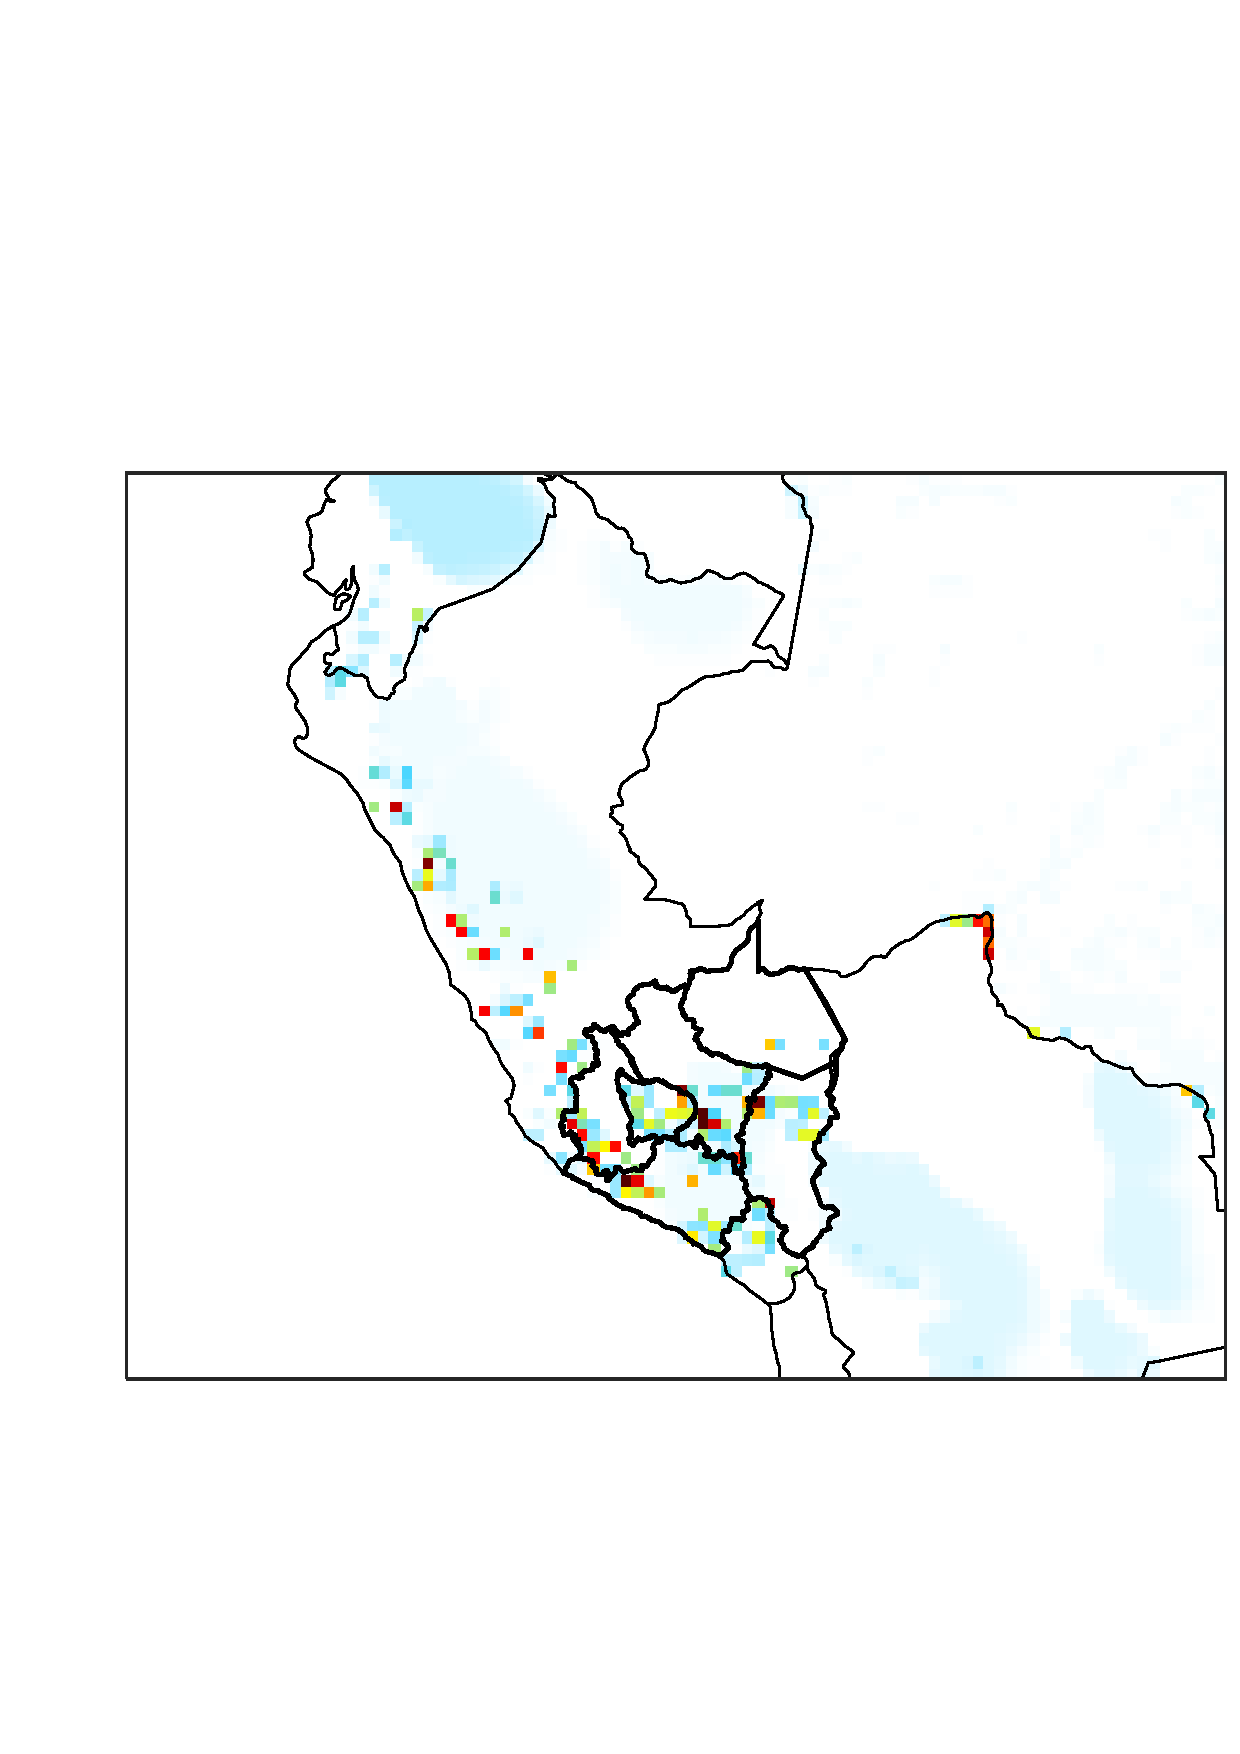
\includegraphics[width = 0.45\linewidth]{templates/figures/Peru_Maps/GMA2018inventory025x025.pdf}} &
\subfloat[GEOS Chem Grid]{\includegraphics[width = 0.45\linewidth]{templates/figures/Peru_Maps/GMA2018inventory2x25.pdf}}\\


\end{tabular}
  
\centering
\captionof{figure}{Map showing how the GMA2018 emission estimates for the year 2015 were distributed in Peru }
\label{fig:GMA2018}
\end{figure}
\FloatBarrier


\begin{flushleft}
For each grid box in the case study region, the emissions were modified from their original GMA 2018 estimates to new values based on Hg emission estimates produced by the Artisanal Gold Council(AGC)
\end{flushleft}

\subsection{Markov Chain Monte Carlo}

\begin{flushleft}
The Markov-Chain Monte Carlo (MCMC) is a sampling method that is also useful for fitting models to data\cite{hogg_data_2018}. We apply the MCMC to constrain ASGM Hg emissions from the case study region in Peru. The basic idea behind this approach is to compare the generated models to the data. The model is generated by a set of parameters and emissions, and we aim to sample from the parameters that best fit our data. The MCMC is used to compare the modeled concentrations to the observed data using metrics such as the $95^{th}$ confidence interval, mean, and the interquartile range. The MCMC generatively models given data by sampling around optimum values from the posterior distribution. The MCMC is a Bayesian approach; hence it requires the definition of priors on the parameters of interest. The priors encode information that we already know of the system. The probability of the model given the observed data is given by the posterior probability, $P(\theta|D)$, which is calculated using the Bayes theorem:

\begin{equation}
\label{bayes_eq}
P(\theta|D)=\frac{P(D|\theta)P(\theta)}{P(D)}
\end{equation}
where:
\end{flushleft}

\begin{description}[leftmargin=!,labelwidth={3 em}]
    \item [$P(D|\theta)$] is the likelihood which is the probability of the data given the model
    \item [$P(\theta)$] is the prior, which is the probability of the model and 
    \item [$P(D)$] is the evidence which is the probability of the data.
\end{description}

\begin{flushleft}
The MCMC enables the estimation of the sampling of the posterior distribution, which is the left-hand side of Equation~\ref{bayes_eq}. The MCMC is set up by following a set of steps that include defining a function that outputs a model given a set of input parameters and establishing an ensemble of walkers defined by a $\theta$ vector that contains a set of parameters from the model generating function. For the model generating function, the Hg concentration at a particular grid box is defined as a linear combination of Hg concentration signals from the case study region and the baseline Hg concentration as shown in the Equation \ref{Hg_conc} below:

\begin{align}
\begin{split}\label{Hg_conc}
Hg_{conc}= {}&Hg_{m(MdD)}+ Hg_{m(S-Puno)} + Hg_{m(N-Puno)} + Hg_{m(Apr)}+ Hg_{m(Aqp)}\\
            & +Hg_{m_0}
\end{split}
\end{align}

where:
\end{flushleft}

\begin{description}[leftmargin=!,labelwidth={5 em}]
    \item [$Hg_{m(MdD)}$] is the Hg concentration signal resulting from emissions from the Madre de Dios (MdD) grid box
    \item [$Hg_{m(S-Puno)}$] is the Hg concentration signal resulting from emissions from the South Puno (S-Puno) grid box
    \item [$Hg_{m(N-Puno)}$] is the Hg concentration signal resulting from emissions from the North Puno (N-Puno) grid box
    \item [$Hg_{m(Apr)}$] is the Hg concentration signal resulting from emissions from the Apurimac (Apr) grid box
    \item [$Hg_{m(Aqp)}$] is the Hg concentration signal resulting from emissions from the Arequipa (Aqp) grid box
    \item [$Hg_{m_0}$] is the baseline Hg concentration signal.
\end{description}

\begin{flushleft}
Each of the $Hg_{m(region)}$ terms of Equation \ref{Hg_conc} represent signals from the different departments are calculated using Equation~\ref{ysignal}. Equation~\ref{ysignal} The $m_(region)$ terms are the only unknowns in  and the equation can be expanded to isolate the terms with $m_(region)$, which is the parameter we are optimizing for in the MCMC method. The expanded form of Equation \ref{Hg_conc} is shown below:

\begin{align}
\begin{split}\label{Cs36PoGd2l}
Hg_{conc}={}& (m_{(MdD)}Hg_{sig_{(MdD)}} -m_oHg_{sig_{(MdD)}})+ (m_{(S-Puno)}Hg_{sig_{(S-Puno)}} -m_oHg_{sig_{(S-Puno)}}) \\
            &+ (m_{(N-Puno)}Hg_{sig_{(N-Puno)}} -m_0Hg_{sig_{(N-Puno)}}) + (m_{(Apr)}Hg_{sig_{(Apr)}} -m_oHg_{sig_{(Apr)}}) \\
            &+ (m_{(Aqp)}Hg_{sig_{(Aqp)}} -m_oHg_{sig_{(Aqp)}})+Hg_{m_0}
\end{split}
\end{align}

Since the values of $m_{(region)}$ are the parameters that we want to estimate using MCMC, they can represented as $\theta_i=m_{(region)}, i=1$ and the other terms including the background concentration are combined into one constant, C:

\begin{equation}
\begin{aligned}
    Hg_{conc}  & = \theta_0C  + \theta_1Hg_{sig_{(MdD)}}+ \theta_2Hg_{sig_{(S-Puno)}} +  \theta_3Hg_{sig_{(N-Puno)}} \\
                & \ \ \ \  +\theta_4Hg_{sig_{(Apr)}} +  \theta_5Hg_{sig_{(Aqp)}}
\end{aligned}
\end{equation}

\begin{align}
Hg_{conc} =\begin{bmatrix} C & Hg_{sig_{(MdD)}} & Hg_{sig_{(S-Puno)}} &Hg_{sig_{(N-Puno)}} &Hg_{sig_{(Apr)}} &Hg_{sig_{(Aqp)}}\end{bmatrix} \times 
            \begin{bmatrix} \theta_0 \\ \theta_1 \\ \theta_2\\ \theta_3\\ \theta_4\\ \theta_5  \end{bmatrix}
\end{align}
where $\theta_0=1$ and $Hg_{conc}$ is the modeled Hg concentration at the observation site of interest.
\end{flushleft}

\begin{flushleft}
The output of 
\end{flushleft}





\section{Results and Discussion}
\subsection{Observed Hg Concentration at CHC}
\begin{flushleft}
The time series of the observed concentration at the CHC station between July 2014 and January 2016 is shown on Figure\ref{fig:ObsTseries}. The detailed characteristics of the observations over this measurement period were described in Koening et al.,(2020); hence our analysis was focused on using the observation TGM data to evaluate the performance of the GEOS-Chem model in predicting the \hg based on the input \hg emission inventories. As shown by the plot of the \hg 120 day moving as a function of time on Figure\ref{fig:ObsTseries}, we found that the observed TGM concentration in the atmosphere had a visible upward trend, which Koening et al.,(2020) attribute to the El Niño-Southern Oscillation (ENSO). Consequently, Koening et al.,(2020) categorized the measured TGM concentrations in the atmosphere at the CHC site into normal conditions (NC), 2014-07 to 2015-05 and ENSO conditions  2015-06 to 2016-01.
\end{flushleft}

\begin{figure}[H]
  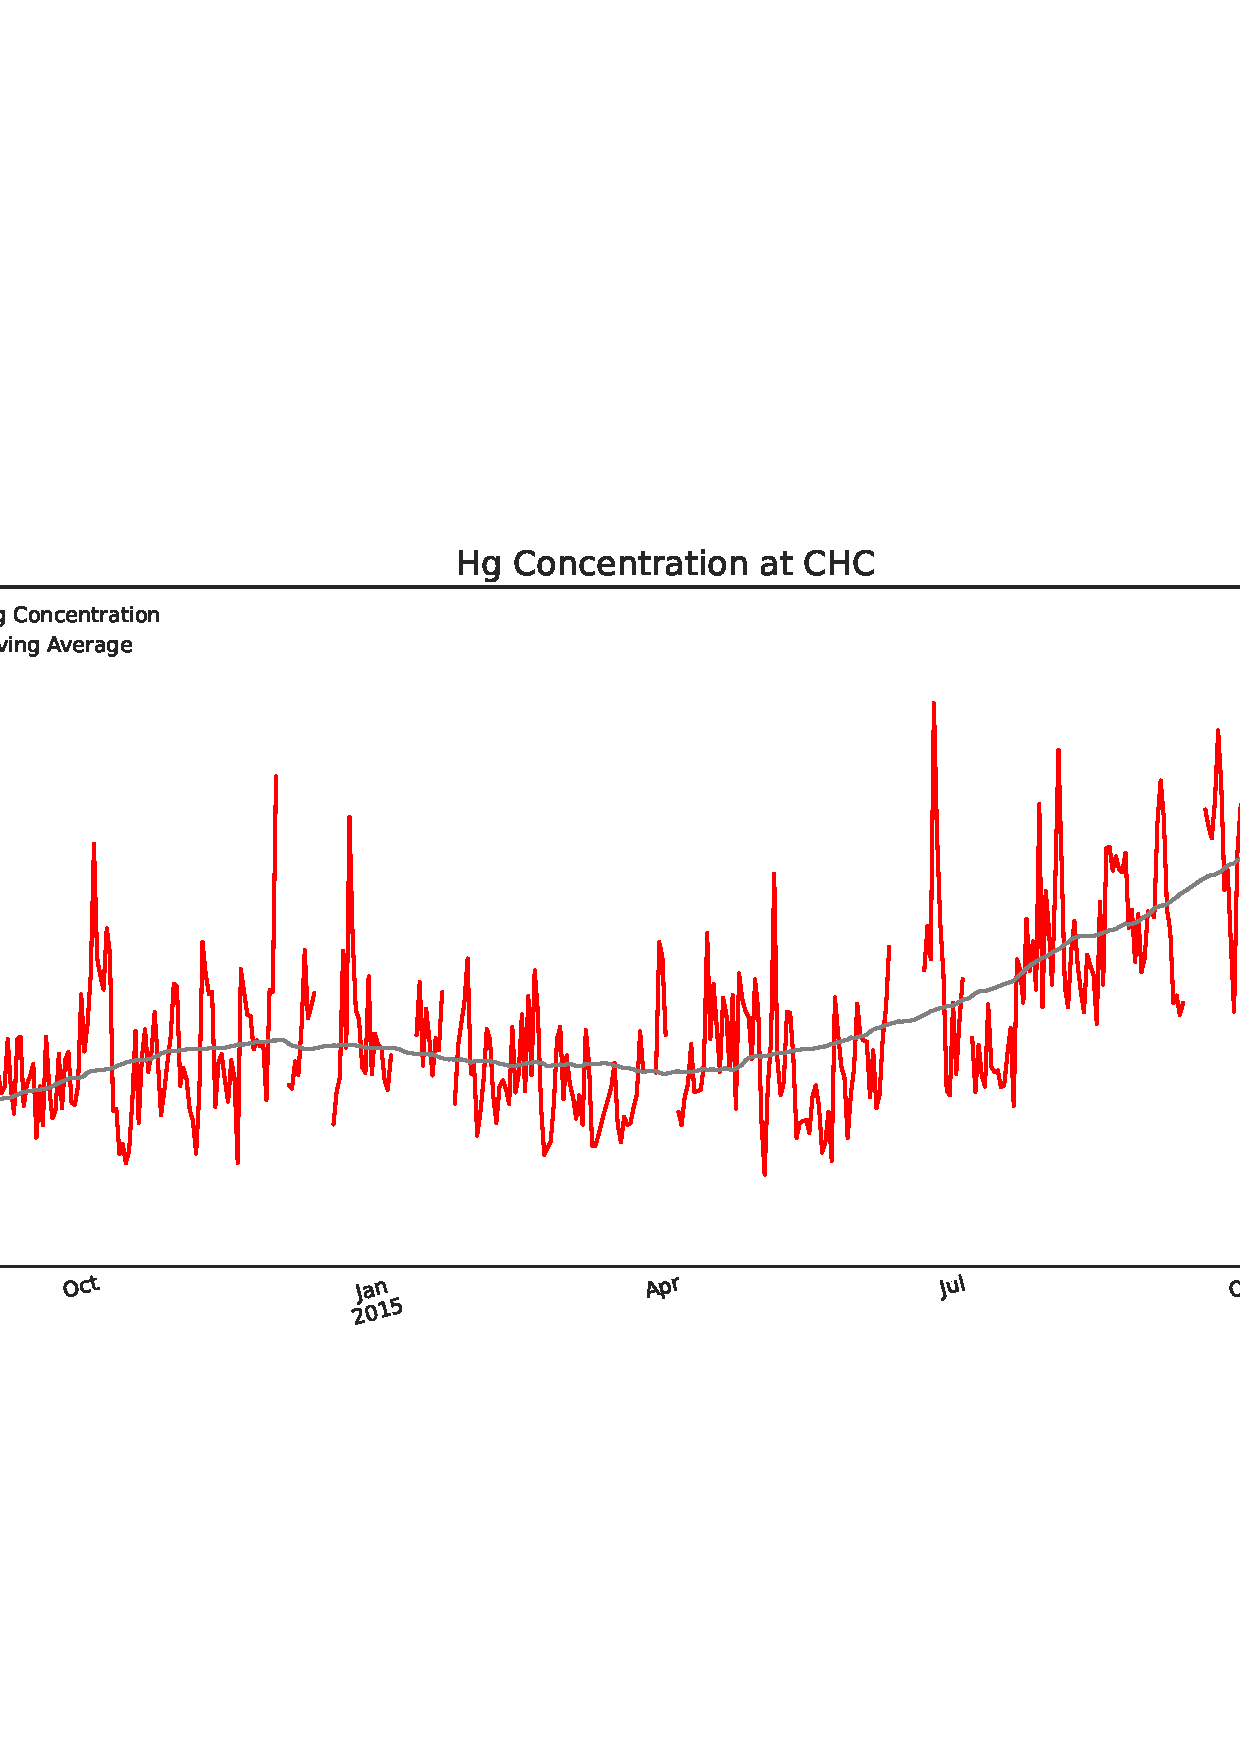
\includegraphics[width=\textwidth]{templates/figures/GMOS_Sites/ObsTimeSeries.pdf}
 
  \caption{The average daily TGM concentration at CHC in ngm\textsuperscript{-3} as a function of time over the measurement period from July 2014 to January 2016. The daily average concentration in indicated by the red line while the grey line shows the 120 day moving average which clearly highlights the upward trend in the daily averages}
  \label{fig:ObsTseries}
  \centering
\end{figure}
\FloatBarrier

\begin{flushleft}
  Figure \ref{fig:ModelvsObsNstats} the detailed comparison between the simulated \hg  and the observed TGM concentration at CHC. The observations (in red) are plotted as a function of time in (a) with the Base (ASGM= OFF) simulation (in green) and (c) with the Base (ASGM= ON) simulation in (blue). The scatter plots in (b) and (d) represent the modeled \hg  as a function of the measured TGM concentration. The scatter plot in plot (b) the variability in the observed TGM concentration is not captured by the Base (ASGM= OFF) simulation while the scatter plot in (d) shows that the Base (ASGM=ON) simulation over estimates the observed values even though it matches the variability in the values. The dispersion around the 1:1 line is substantial in both scatter plots and hence the correlation coefficient is low in both cases. 
\end{flushleft}


\begin{figure}[H]
  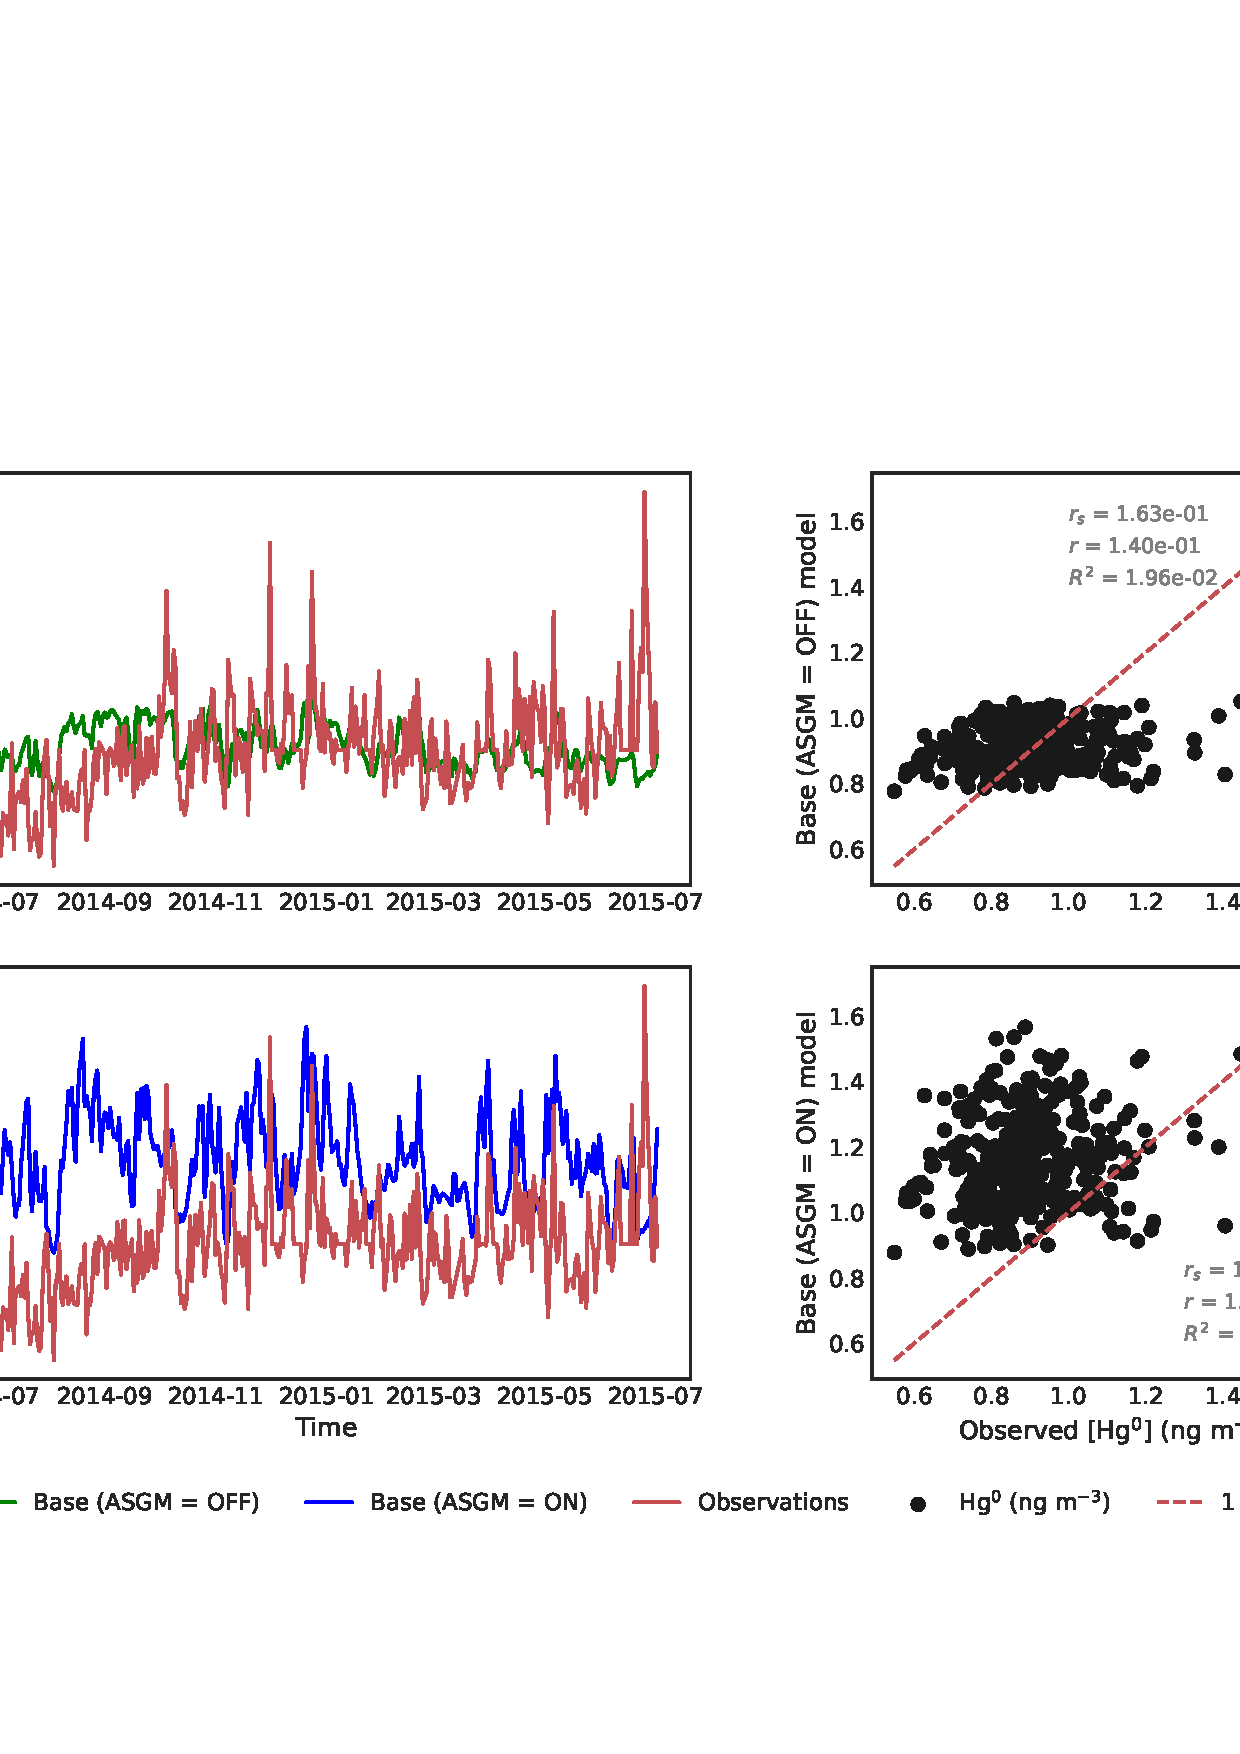
\includegraphics[width=\textwidth]{templates/figures/ModelvsObs/TimeSeriesNsactter_obsVmodel_v1.pdf}
  \centering
  \caption{Observed vs modelled (3 different simulations) Hg concentration at CHC and scatter plots of how the model compares with the observations  }
  \label{fig:ModelvsObsNstats}
\end{figure}
\FloatBarrier
\begin{flushleft}
We also found that the mean \hg concentration produced by the Base (ASGM= OFF) simulation was within 1\% of the observed TGM concentration as seen on Table \ref{tab:ModelvsObsStats} where $\mu$ is the annual average Hg concentration, $\sigma$ is the standard deviation, $iqr$ is the interquartile range, $r_s$ is the Spearman correlation, $r$ is the Pearson correlation, and $R^2$ is the coefficient of determination. On the contrary, the average \hg produced by the \on shown by the blue line plot on Figure \ref{fig:ModelvsObsNstats} overestimated the mean by 29\%.
 
\end{flushleft}
\setlength{\tabcolsep}{2.5pt}
\begin{table}[H]
  \begin{center}
    \caption{Characteristics of observed and modelled Hg concentration in CHC where$\mu$ is the annual average Hg concentration, $\sigma$ is the standard deviation, $iqr$ is the interquartile range, $r_s$ is the Spearman correlation, $r$ is the Pearson correlation and $R^2$ is the coeeficient of determination}
    \label{tab:ModelvsObsStats}
    \begin{tabular}{lcccccc}
       %<-- added & and content for each column
      
                          & $\mu$                 & $\sigma$            & $iqr$               & & & \\
                          &  (ng m$^{-3}$)/year)  & (ng m$^{-3}$)/year) & (ng m$^{-3}$)/year) & & & \\
     \cmidrule{2-4}
     Observations         & 0.90             & 0.16            & 0.18        &  & & \\
     \textbf{Simulations} &                  &                  &               &\textbf{$r_s$} &\textbf{$r$} &\textbf{$R^2$}\\ %
      \hline
      Base (ASGM=OFF)     & 0.91             & 0.06            & 0.11         & 0.17         & 0.144      & 0.0196\\ 
      Base (ASGM=ON)      & 1.16            & 0.14            & 0.20        & 0.124         & 0.101       & 0.0102\\ % <--
    \end{tabular}
  \end{center}
\end{table}
\FloatBarrier

\begin{flushleft}
Even though GEOS-Chem reproduced the mean Hg concentrations at CHC in the \off, the Spearman ($r_s$) and Pearson ($r$) correlations between the modeled and observed concentrations were very low at 1.63e-1 and 1.40e-1, respectively. Moreover, the coefficient of determination, $R^2$ between the observed and modeled concentrations in \on the case was almost zero at 0.021. Also, the \on did not reproduce the variability in the observed concentrations as evident in Figure \ref{fig:ModelvsObsNstats} and in Table \ref{tab:ModelvsObsStats} where we gleaned that the observations had more than twice the modeled variance in the \on the case. Brasseur and Jacob (p.471 2017) assert that in cases where a model captures the observed means but not the observed variability, the mean may be wrongly interpreted \cite{brasseur_modeling_2017}. In the case of \off, the mean may be wrongly interpreted because of the exclusion of the ASGM Hg emissions. In addition, we found that turning on ASGM emissions in GEOS-Chem led to  atmospheric Hg concentrations that had a variance comparable with the observed variance. However, we also discovered that turning on ASGM emissions in the model did not improve the correlation between the modeled and observed \hg in the atmosphere. 
The relationship between the mean and variance in the observed and modeled  atmospheric Hg concentration at CHC was further explored as shown in Figure \ref{fig:Histplots} which shows the extent to which the GEOS-Chem model reproduces the mean and IQR of the observations. Even though the \on  better recreated the IQR of the Hg concentration in the atmosphere, the mean \hg in this simulation was almost two standard deviations away from the mean of the observations. The above comparison indicates that the mean was not a good metric to investigate the relationship between the Hg concentration in the atmosphere and ASGM emissions as modeled by GEOS-Chem. 
\end{flushleft}



\begin{figure}[H]

\begin{tabular}[H]{cc}

\subfloat[]{\includegraphics[width = 0.5\linewidth]{templates/figures/ModelvsObs/06-12-22_models_vs_observations_density-plot.pdf}} &
\subfloat[]{\includegraphics[width = 0.5\linewidth]{templates/figures/ModelvsObs/06-12-22_models_vs_observations_density-plot_std.pdf}}
\end{tabular}
\centering
\captionof{figure}{Plots Showing Data and Modeling  Results from GMOS Monitoring Network Sites in South America}
\label{fig:Histplots}
\end{figure}
\FloatBarrier

\begin{flushleft}
Instead, the IQR and 95$^{th}$ percentile range were found to be informative metrics about the effect of ASGM on the simulated Hg concentration site at a distant high altitude measuring station site. The failure of GEOS-Chem to reproduce the observed mean Hg concentration at a high altitude measuring site may be attributed to the model's poor parameterizations, such as the influence of dry deposition. The flaws in the GEOS-Chem Hg dry deposition scheme in version 12.8.1 of the GEOS-Chem used in this analysis were discussed in detail and improved in Feinberg et.al (2022). Furthermore, we hypothesized that the poor spatial distribution of emissions in the 2015 Hg ASGM emissions inventory, which are input to the GEOS-Chem, may have also contributed to the model observation mismatches. 

\end{flushleft}

\subsection{Markov Chain Monte Carlo Simulation }
\renewcommand{\arraystretch}{2}

    
\begin{table}[H]
\caption{Table showing the emission estimates for each of the grid boxes in the case study region when the $95^{th}$ percentile range is used as the metric to compare the model outputs to observations}
    \label{tab:MCMC_estimates}
\begin{tabular}{lc}

\textbf{Region}        & \textbf{Emission Estimate}                             \\
\hline
Madre de Dios & $16.97^{+21.27}_{-12.27}$ \\

Apurimac      & $14.90^{+16.16}_{-10.53}$\\

Arequipa      & $32.83^{+34.94}_{-24.31}$ \\

North Puno    & $13.44^{+17.51}_{-10.07}$ \\

South Puno    & $06.51^{+7.26}_{-4.72}$ \\
\hline
\end{tabular}
\centering
\end{table}

\begin{figure}[H]
  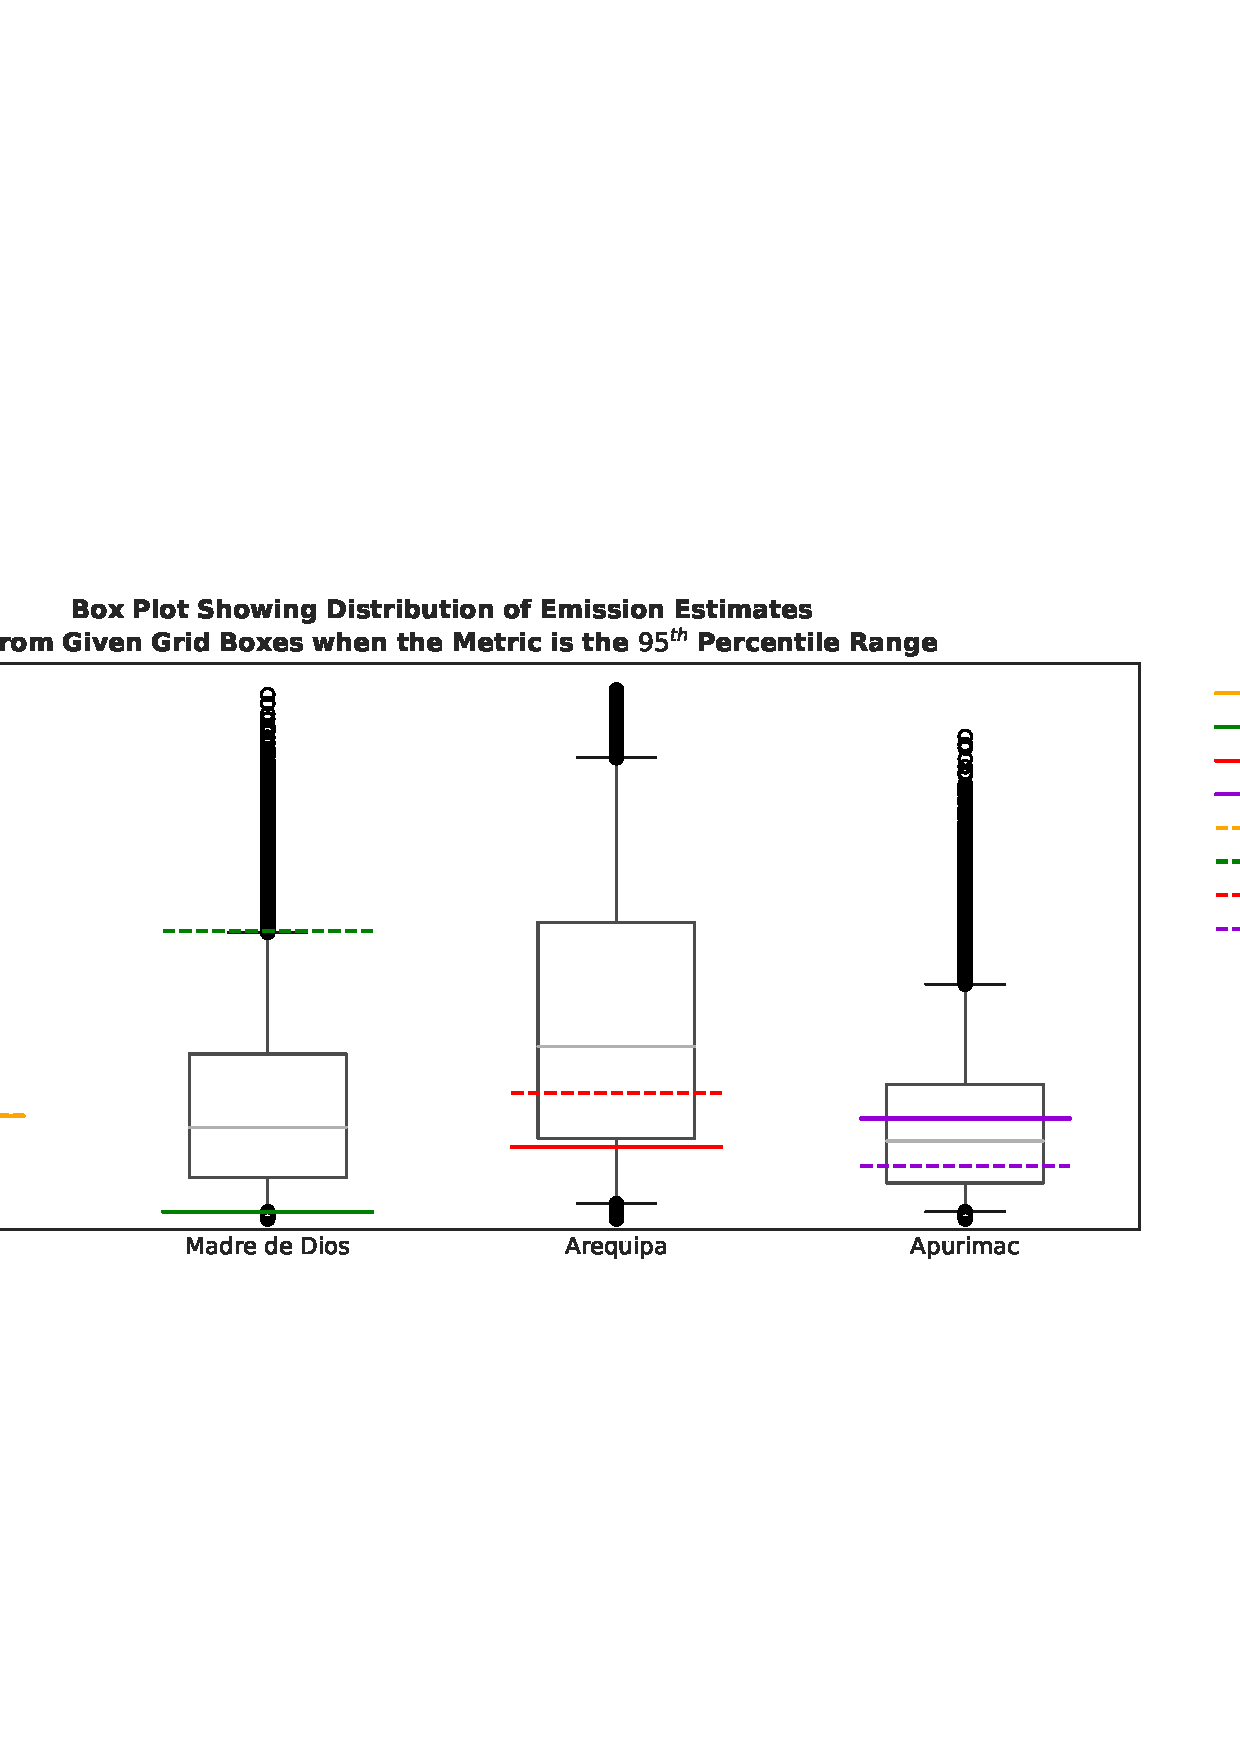
\includegraphics[width=\textwidth]{templates/figures/MCMC/MCMCMCMC_Estimates95th.pdf}
  \centering
  \caption{Emission Estimates when the $95^{th}$ percentile range is used as the metric to compare the model outputs to observations }
  \label{fig:MCMC_estimatesiqr}
\end{figure}
\FloatBarrier

\begin{figure}[H]
  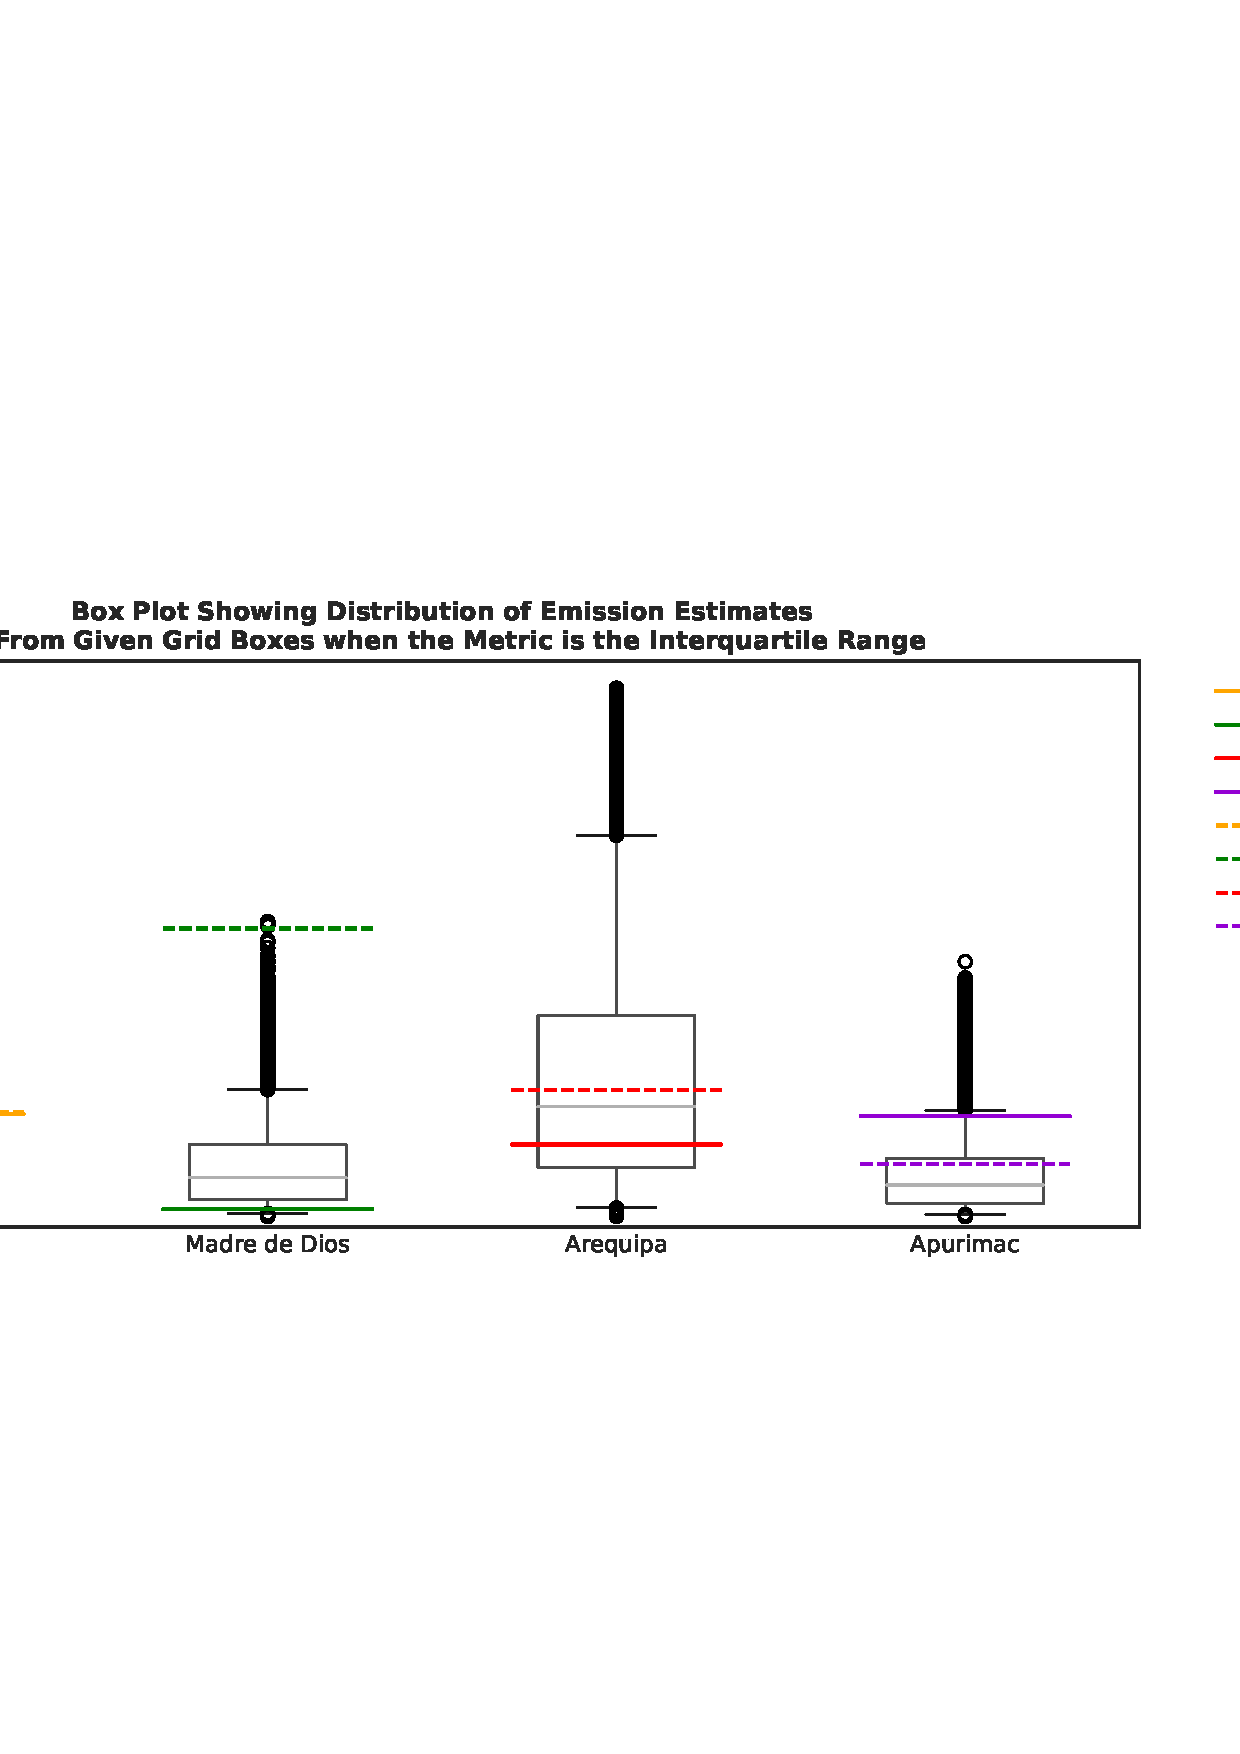
\includegraphics[width=\textwidth]{templates/figures/MCMC/MCMCMCMC_Estimatesiqr.pdf}
  \centering
  \caption{Emission Estimates when the IQR is used as the metric to compare the model outputs to observations }
  \label{fig:MCMC_estimates95}
\end{figure}
\FloatBarrier
\begin{flushleft}

\end{flushleft}



\subsection{Another subsection sample}
\section{Policy Implications}